\section{Design and Implementation}

Figure \ref{fig:comms_network_map} shows the new network layout for Tiberius III. The new network has been designed for long range, high reliability and low power, while maintaining an easy to use architecture that makes it easy to connect to devices no matter where they reside.
\subsection{Overall communications system design}
\begin{figure}[!htb]
\begin{center}
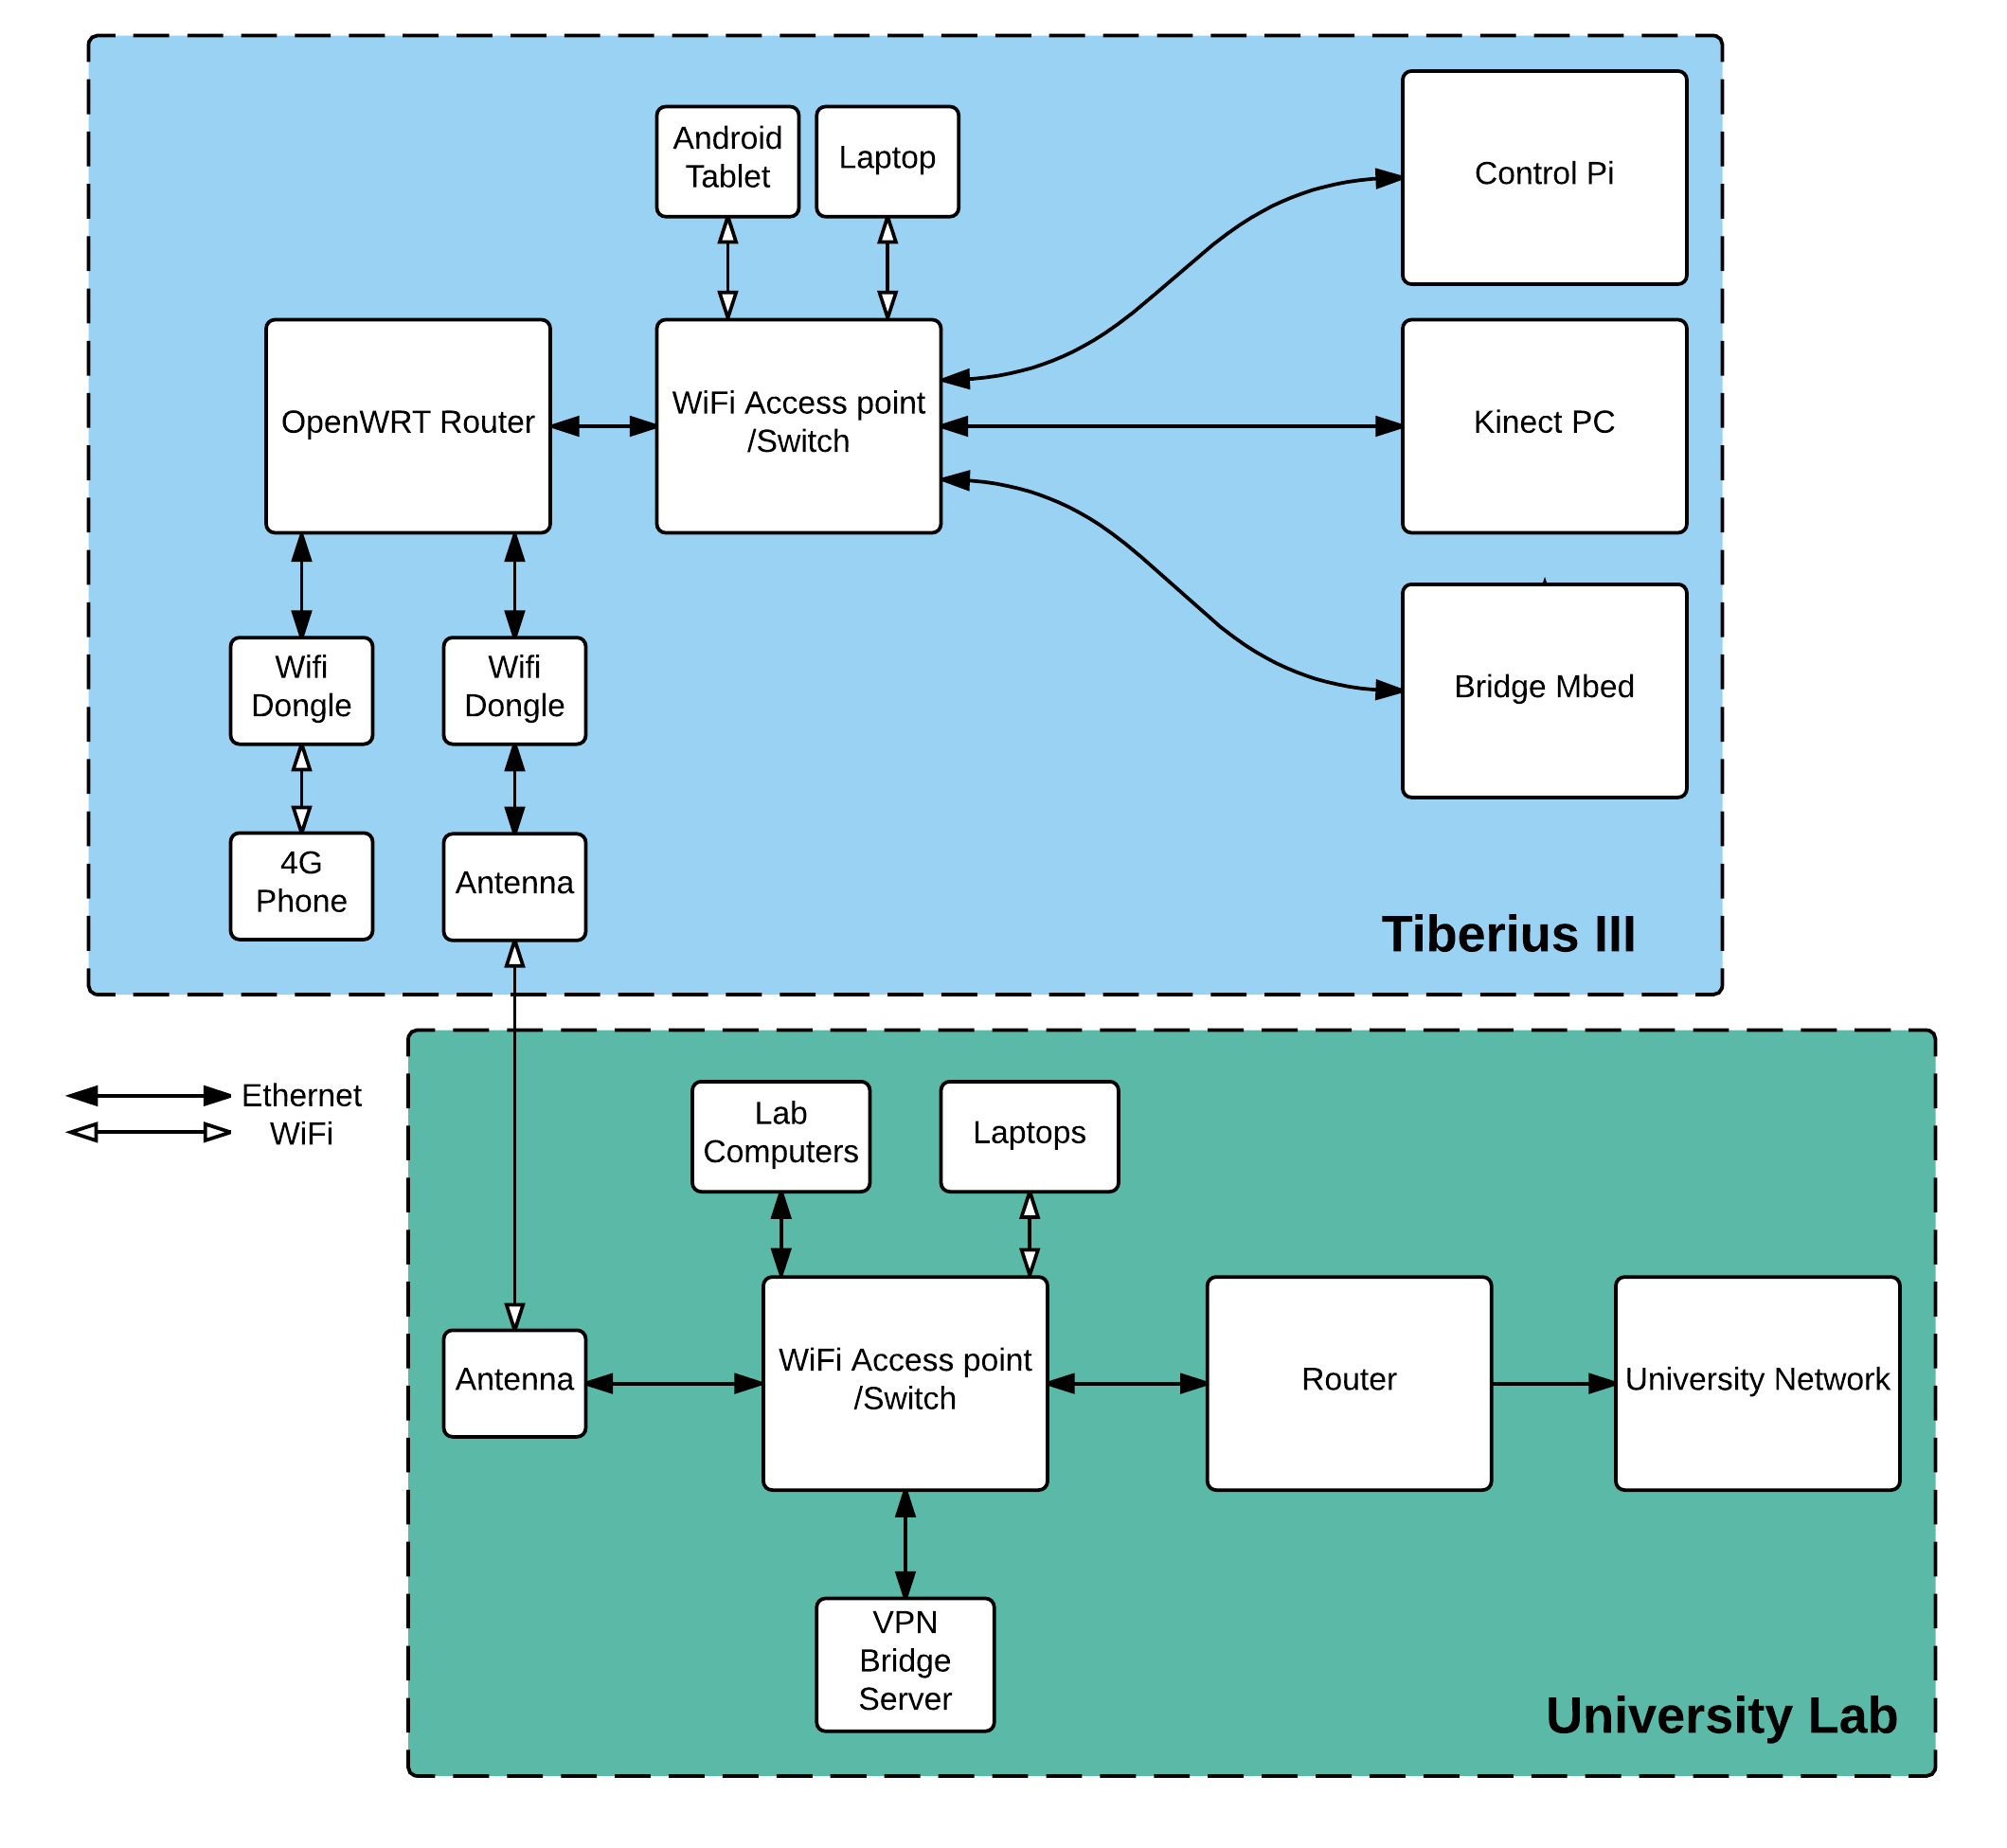
\includegraphics[width=15cm]{comms_network_map.png}
\end{center}
\caption{Communications Network Map}
\label{fig:comms_network_map}
\end{figure}




\subsubsection{Self Aiming Wi-Fi Link}
In order to facilitate a long range Wi-Fi link, long range highly directional antennas had to be used. Since the chosen antennas only have a 30 degree cone of signal  a system to point the antennas at each other was required.

The antenna in the university lab is pointed in the general direction that Tiberius will be operated in. It can easily be adjusted by hand and will not be rotating so it made little sense to make it self aiming.

The antenna on Tiberius III is able to automatically aim at the GPS location of the antenna in the lab. This means that both antennas will always be facing each other no matter what direction Tiberius is travelling in. In order to aim at the GPS point, the antenna is mounted on a pylon to raise it above the rest of the chassis and can be rotated using a servo. The servo is connected to control pi using the External Hardware Controller (An Arduino Mega which interfaces with any additional hardware that need to be directly controlled by the control pi).

\subsubsection{4G Connection using Mobile Phone}
Since mobile phones are an extremely easy way to get a 4G connection, it seemed logical to use one to provide a simple way of adding 4G connectivity to Tiberius III. In order for the internet connection to be used the phone needs to be running a portable Wi-Fi hotspot with the name "Tiberius-4G". The OpenWRT router will automatically connect to the network provided by the phone and use it as a failover internet connection in case the Wi-Fi connection is lost.

\subsubsection{OpenWRT router}
At the core of the new networking system on Tiberius III is a Raspberry Pi running OpenWRT open-source router software. This was required since a special network interface card was needed in order to use the directional antenna to its full potential. It also allows for other connections to be added in the future. In addition it also provides the essential failover capability for the Wi-Fi and 4G connections.

\subsubsection{VPN failover}
The failover capability is mostly provided by the OpenWRT router which will automatically route packets through another WAN interface if it loses Wi-Fi. This behaviour was achieved by setting the metrics on both Interfaces within OpenWRT.

\subsubsection{Local Wi-Fi Access Point and switch}
The Wi-Fi access point is an essential component for outdoor testing, since it removes the requirement for a network cable between a laptop and Tiberius. It also allows for lots of devices to be connected to Tiberius as it is moving around without the need for extra switches and cabling. When testing outdoors it is often very useful to have an internet connection, Tiberius can  provide any device connected access to the internet through its own long range communications system.

\subsubsection{VPN Bridge} 
One of the biggest challenges with a multi-network system is how to maintain communication between devices when they could be behind several firewalls or routers with no specific routes defined between devices.

This leads to the single most important part of the new networking system, the VPN, which removes almost all the headaches of networking for developers. It seamlessly bridges all the various networks associated with Tiberius together over the internet. This allows a user in the university lab to stay connected to a device on Tiberius III even when operating on 4G. The VPN can bridge through firewalls and port restrictions to provide a continuous connection irrespective of the routes or subnets involved.

\subsubsection{Subnets and IP allocations}
To further simplify the problem it was decided that all devices in the lab and on Tiberius would have assigned IP addresses and be on the same subnet. This makes it much easier from the standpoint of remembering addresses of devices and allows different Tiberius's to communicate with each other easily.

The 10.113.211.0 subnet was used for all devices meaning that users would only have to remember one number for each device. Or they could look the address up on the allocations spreadsheet.


\subsection{Software setup}
\subsubsection{OpenWRT router}
Some screenshots of the configuration?
\subsubsection{SoftEther VPN Bridge}
Diagram of how the network appears to devices when using the bridge
\subsubsection{Device Settings}
Not sure if I need this

\subsection{Hardware setup}
\subsubsection{Wiring diagram}
Not sure if I need this
\subsubsection{Self Aiming Wi-Fi antenna}
Explaination of how the antenna is aimed or something



